%-------------
% Metodologia 

% Capítulo de materiais e métodos. Materiais é tudo aquilo que foi usado, desde recurso de hardware, notebook, bancada, motor, contator etc. Método é a descrição da ideia e sua implementação
%-------------
\chapter{Metodologia} \label{Metodologia}
O desenvolvimento deste trabalho foi estruturado em etapas complementares, abrangendo fundamentação teórica, análise exploratória de dados, aquisição experimental de medições elétricas, modelagem de algoritmos de aprendizado de máquina, implementação do sistema elétrico e validação experimental.

Inicialmente, foi realizada uma revisão bibliográfica com o objetivo de fundamentar a aplicação de redes neurais artificiais na análise de sistemas elétricos, com ênfase em modelos do tipo Multilayer Perceptron (MLP). Também foram investigadas abordagens relacionadas à execução de modelos de aprendizado de máquina próximos à fonte de dados, no contexto de aplicações de Internet das Coisas, visando possibilitar processamento e inferência em tempo real. Foram analisados trabalhos voltados à estimativa do fator de potência, à classificação de tipos de carga e à aplicação de técnicas de aprendizado de máquina em sistemas elétricos, estabelecendo a base conceitual e metodológica desta pesquisa.

Paralelamente à fundamentação teórica, foi realizada uma análise exploratória de dados utilizando a base residencial \textit{Individual Household Electric Power Consumption}, disponibilizada no repositório \textit{UC Irvine Machine Learning Repository}. Essa etapa teve como objetivo investigar o comportamento das grandezas elétricas e sua relação com o fator de potência, permitindo identificar as variáveis mais relevantes para representação do comportamento das cargas elétricas e para a estimação do fator de potência. As variáveis selecionadas foram posteriormente utilizadas como entradas nos modelos de aprendizado de máquina desenvolvidos neste trabalho.

Na etapa experimental, foi desenvolvido um sistema de aquisição de dados elétricos utilizando o sensor PZEM-004T. Na sequência, procedeu-se à modelagem das redes neurais, contemplando as etapas de treinamento e teste no ambiente Edge Impulse e validação do sistema, por meio de métricas adequadas de avaliação de desempenho. Posteriormente os modelos foram integrados ao fluxo de processamento implementado na plataforma Node-RED, responsável pela execução das inferências em tempo real. Por fim, foi implementado um painel de monitoramento para visualização e acompanhamento em tempo real das grandezas elétricas medidas e estimadas.

%------------------------------------------------------------------
%------------------------------------------------------------------
\section{Visão Geral do Sistema Proposto}

Para o desenvolvimento do sistema proposto foram seguidas as seguintes etapas:

\begin{enumerate}
    \item \textbf{Definição dos Componentes:} Nesta etapa foram selecionados os elementos de hardware necessários para a aquisição e transmissão dos dados elétricos. Foram utilizados o sensor PZEM-004T para medição das grandezas elétricas e o microcontrolador NodeMCU ESP8266 para coleta dessas leituras e transmissão dos dados para o ambiente de processamento Node-RED.
    
    \item \textbf{Definição da Arquitetura do Sistema:} Foi projetada a arquitetura funcional do sistema, estabelecendo o fluxo de dados desde a aquisição das variáveis elétricas até o processamento, implementação dos modelos e visualização dos resultados. Nesta fase foram definidos os módulos de aquisição de dados, comunicação via protocolo MQTT, inferência do modelo de aprendizado de máquina e interface de monitoramento.
    
    \item \textbf{Análise das Características das Cargas Elétricas:} Esta etapa consistiu no estudo do comportamento elétrico de diferentes tipos de cargas, considerando a relação entre tensão, corrente, potência ativa, potência reativa, potência aparente e fator de potência. Essa análise fundamentou a escolha das variáveis de entrada para os modelos.
    
    \item \textbf{Coleta de Dados em Cenários Reais:} Realizou-se a aquisição de dados elétricos em ambiente laboratorial, utilizando diferentes configurações de carga. Essa etapa teve como objetivo construir a base de dados utilizada no treinamento e validação do modelo de classificação.
    
    \item \textbf{Treinamento do Modelo de Classificação:} Envolveu o treinamento por meio da plataforma Edge Impulse e conversão dos modelos para o formato WebAssembly, possibilitando a execução no ambiente Node-RED.
    
    \item \textbf{Processamento dos Modelos:} Realização da exportação e integração dos modelos ao ambiente de processamento Node-RED, permitindo a execução da inferência em tempo real a partir dos dados medidos pelo sensor.
    
    \item \textbf{Comunicação:} Consistiu na implementação da conectividade entre o microcontrolador e o Node-RED por meio do protocolo MQTT, garantindo a atualização contínua dos dados coletados.
    
    \item \textbf{Criação do Dashboard de Monitoramento:} Desenvolvimento de uma interface gráfica utilizando a plataforma Node-RED, permitindo a visualização em tempo real das grandezas elétricas medidas, da classificação das cargas identificadas e estimativa do PF pelos modelos.
\end{enumerate}

A Figura \ref{fig:integracao_sistema} ilustra a estrutura de funcionamento do sistema proposto.

\begin{figure}[!htbp] 
    \centering 
    \caption{Estrutura funcional do sistema.} 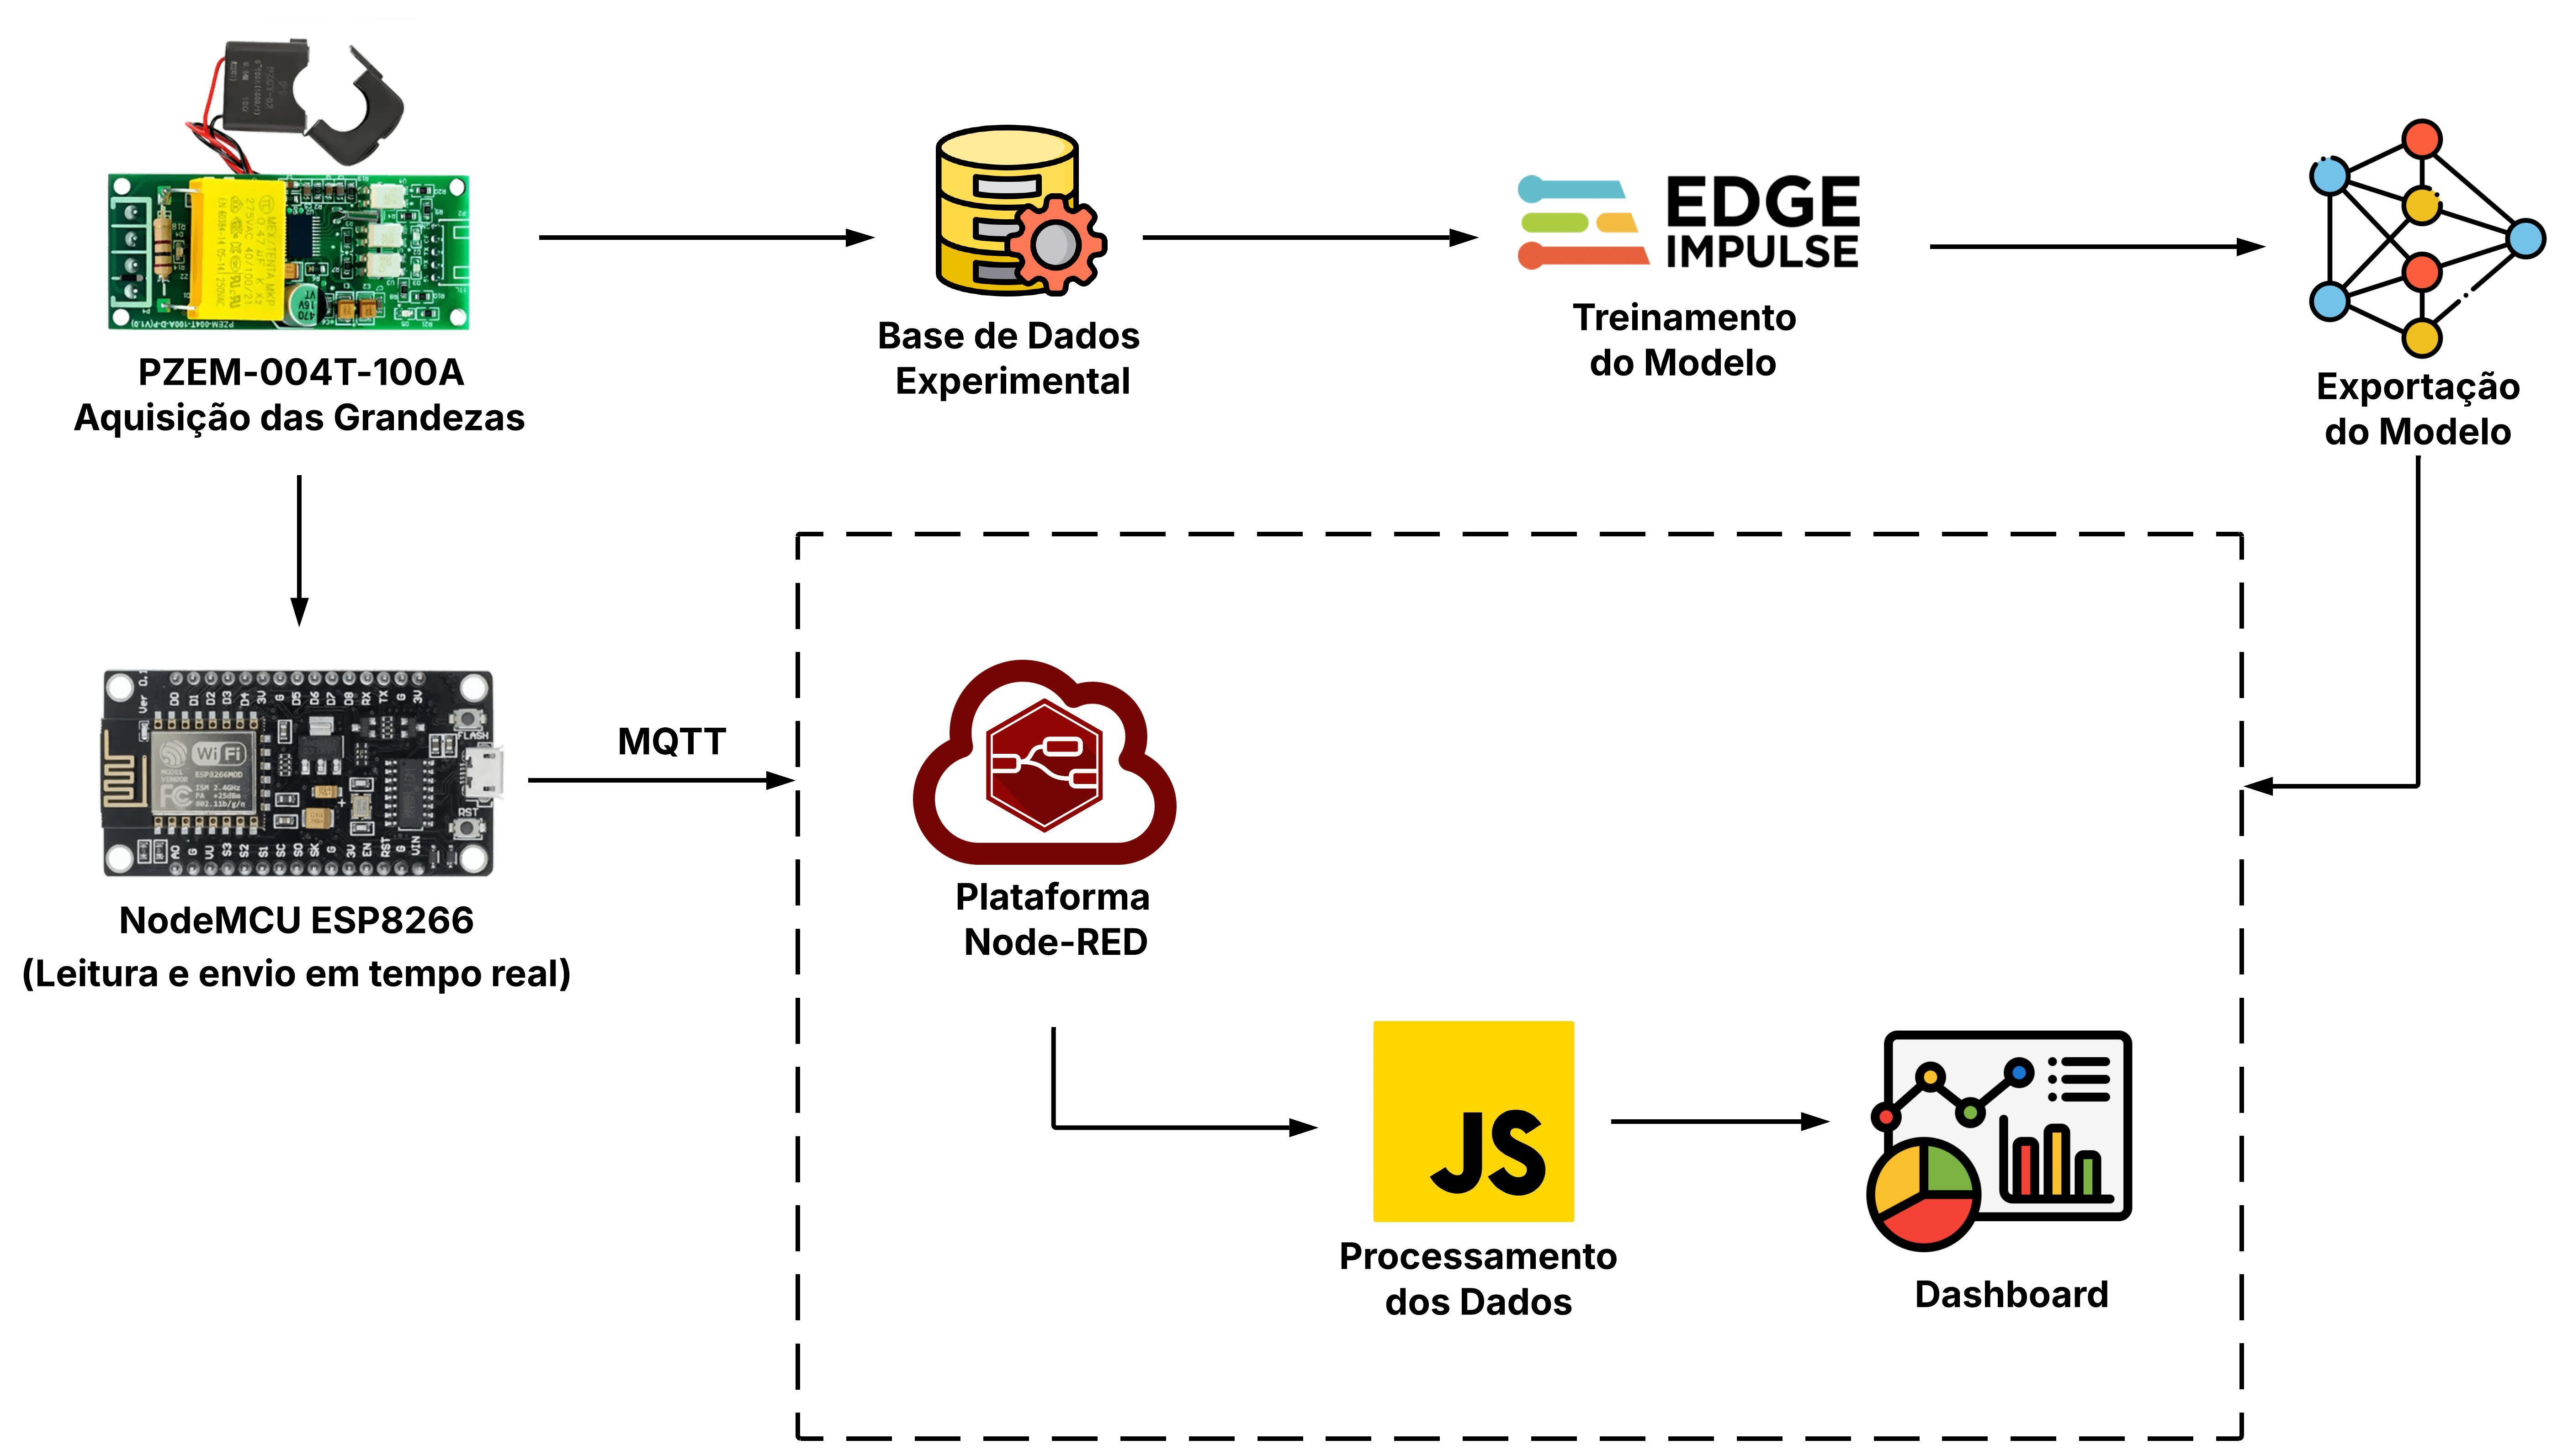
\includegraphics[width=1\textwidth]{Figuras/Integracao do sistema.jpeg} 
    \fonte{\me{2026}} 
    \label{fig:integracao_sistema} 
\end{figure}

%------------------------------------------------------------------
%------------------------------------------------------------------
\section{Materiais}
\subsection{Sensor de medição das grandezas elétrica}

Para a aquisição das grandezas elétricas necessárias ao treinamento e validação dos modelos, bem como para a visualização em tempo real dessas grandezas no painel de monitoramento, foi adotado o módulo de medição PZEM-004T-100A, mostrado na Figura \ref{fig:Medidor PZEM}. Este sensor permite a leitura de multiparâmetros elétricos em tempo real, como frequência, tensão, corrente, potência ativa, energia acumulada e fator de potência, sendo amplamente empregado em aplicações que exigem medições precisas e estáveis, como monitoramento de consumo energético.

\begin{figure}[!htbp] 
    \centering 
    \caption{Módulo PZEM-004T-100A.} 
    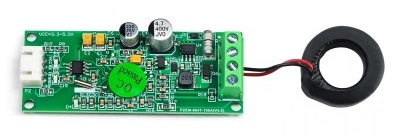
\includegraphics[width= 0.6\textwidth]{Figuras/PZEM.jpg} 
    \fonte{Extraída de \citeonline{UsinaInfo}.} 
    \label{fig:Medidor PZEM} 
\end{figure}

O módulo realiza medições em sistemas monofásicos e possui uma interface de comunicação serial TTL (\textit{Transistor-Transistor Logic} do tipo UART (\textit{Universal Asynchronous Receiver-Transmitter}), que utiliza apenas dois fios (TX e RX) para transmissão serial assíncrona, ou seja, de forma sequencial, bit a bit, sem necessidade de um sinal de clock compartilhado. Essa característica garante simplicidade e eficiência na troca de informações, facilitando a integração com microcontroladores. A Tabela \ref{tab:pzem_especificacoes} apresenta as principais especificações técnicas do sensor utilizado.

\begin{table}[!htbp]
    \centering
    \caption{Especificações técnicas do sensor PZEM-004T-100A.}
    \label{tab:pzem_especificacoes}
    \begin{tabular}{|l|c|c|}
    \hline
    \multicolumn{1}{|c|}{\textbf{Grandezas}} & \textbf{Faixa de Medição} & \textbf{Precisão (\%)} \\
    \hline
    Tensão &            80 – 260 V &        0.5 \\
    Corrente &          0 – 100 A &         0.5 \\
    Potência ativa &    0 – 23 kW &         0.5 \\
    Fator de Potência & 0,00 - 1,00 &       1.0 \\
    Energia &           0 - 9999,99 kWh &   0.5 \\
    Frequência &        45 – 65 Hz &        0.5 \\
    \hline
    \end{tabular}
    \fonte{\me{2026}}
\end{table}

Um dos grandes diferenciais deste módulo é a medição de corrente sem contato direto, feita por meio de um transformador de corrente (TC) incluso, capaz de medir até 100A AC. Diante disso, o sensor PZEM foi escolhido devido  à sua facilidade de integração, baixo custo, excelente desempenho nas medições e comunicação serial simplificada, reduzindo a complexidade do hardware.

%------------------------------------------------------------------
\subsection{NodeMCU ESP8266}
Na aquisição e transmissão dos dados elétricos foi utilizado o microcontrolador NodeMCU ESP8266, apresentado na Figura \ref{fig:nodemcu}. Este dispositivo é amplamente utilizado em aplicações de Internet das Coisas (IoT), pois integra conectividade Wi-Fi nativa, permitindo a comunicação direta com redes sem fio.

\begin{figure}[!htbp] 
    \centering
    \caption{Placa NodeMCU ESP8266.} 
    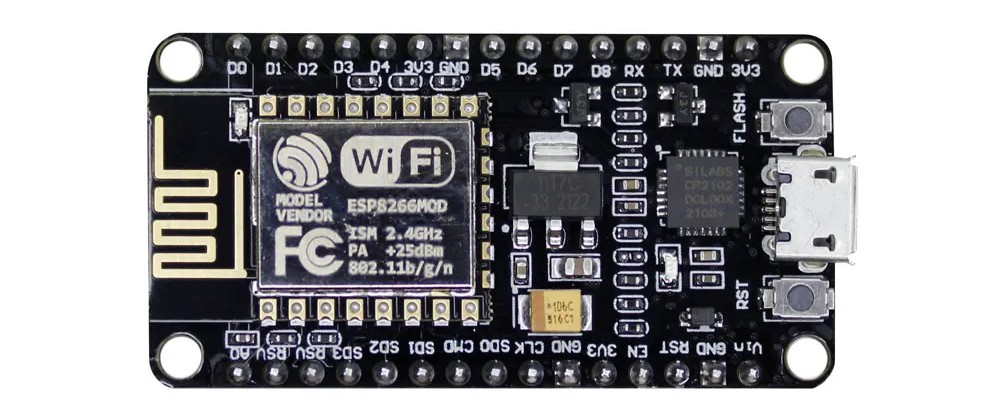
\includegraphics[width=0.6\textwidth]{Figuras/nodeMCU.jpg} 
    \fonte{Figura extraída de \citeonline{kevsrobots_esp8266}.} 
    \label{fig:nodemcu} 
\end{figure}

Conforme apresentado na Tabela \ref{tab:nodemcu_especificacoes} o NodeMCU é baseado no microcontrolador ESP8266, que possui arquitetura de 32 bits e capacidade de processamento adequada para aplicações de baixo custo. Sua principal vantagem é a integração de conectividade Wi-Fi, permitindo a transmissão dos dados coletados para plataformas de processamento e monitoramento em rede.

No sistema desenvolvido, o NodeMCU foi responsável pela leitura dos dados provenientes do sensor PZEM-004T por meio de comunicação serial e pelo envio dessas informações para o ambiente Node-RED utilizando o protocolo MQTT.

\begin{table}[!htbp]
    \centering
    \caption{Especificações técnicas do NodeMCU ESP8266}
    \label{tab:nodemcu_especificacoes}
    \begin{tabular}{|l|c|}
    \hline
    \multicolumn{1}{|c|}{\textbf{Parâmetro}} & \textbf{Especificação} \\
    \hline
    Microcontrolador & ESP8266 \\
    Arquitetura & 32 bits \\
    Frequência de operação & até 80 MHz \\
    Memória Flash & até 4 MB \\
    Conectividade & Wi-Fi 802.11 b/g/n \\
    Tensão de operação & 3,3 V \\
    GPIO & até 11 pinos de entrada/saída \\
    Interface de comunicação & UART, SPI, I2C \\
    \hline
    \end{tabular}
    \fonte{\me{2026}}
\end{table}

%------------------------------------------------------------------
\subsection{Módulo Relé}
O módulo relé, ilustrado na Figura \ref{fig:Modulo_Rele}, é um dispositivo de comutação eletromecânica que permite controlar circuitos de maior potência por meio de sinais de baixa potência provenientes do microcontrolador.

\begin{figure}[!htbp] 
    \centering
    \caption{Módulo relé utilizado para acionamento das cargas.} 
    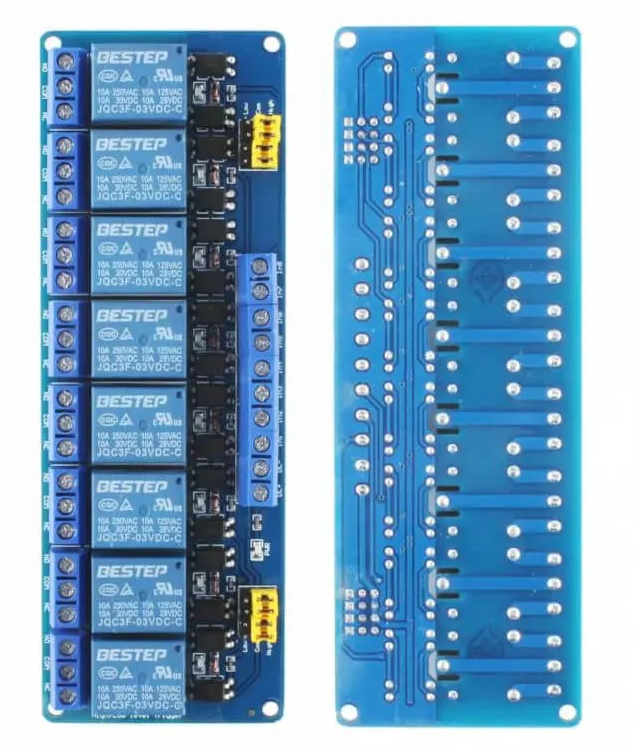
\includegraphics[width= 0.4\textwidth]{Figuras/rele8canais.png} 
    \fonte{Figura extraída de \citeonline{smartkits_rele8ch}.} 
    \label{fig:Modulo_Rele} 
\end{figure}

No sistema desenvolvido, o módulo relé foi empregado para o controle das cargas elétricas utilizadas nos experimentos, sendo acionado por sinais digitais gerados pelo microcontrolador. Quando ativado, o relé altera o estado de seus contatos internos, permitindo ou interrompendo a passagem de corrente no circuito de potência.

%------------------------------------------------------------------
\subsection{Contatores}
São dispositivos de comutação projetados para operar em circuitos de potência, sendo capazes de suportar correntes mais elevadas e maior número de ciclos de operação quando comparados a relés convencionais. Seu funcionamento baseia-se na atuação de um eletroímã que, ao ser energizado, aciona mecanicamente os contatos responsáveis pela abertura ou fechamento do circuito elétrico, conforme apresentado na Figura \ref{fig:Contactor}.

\begin{figure}[!htbp] 
    \centering
    \caption{Contator utilizado no sistema experimental.} 
    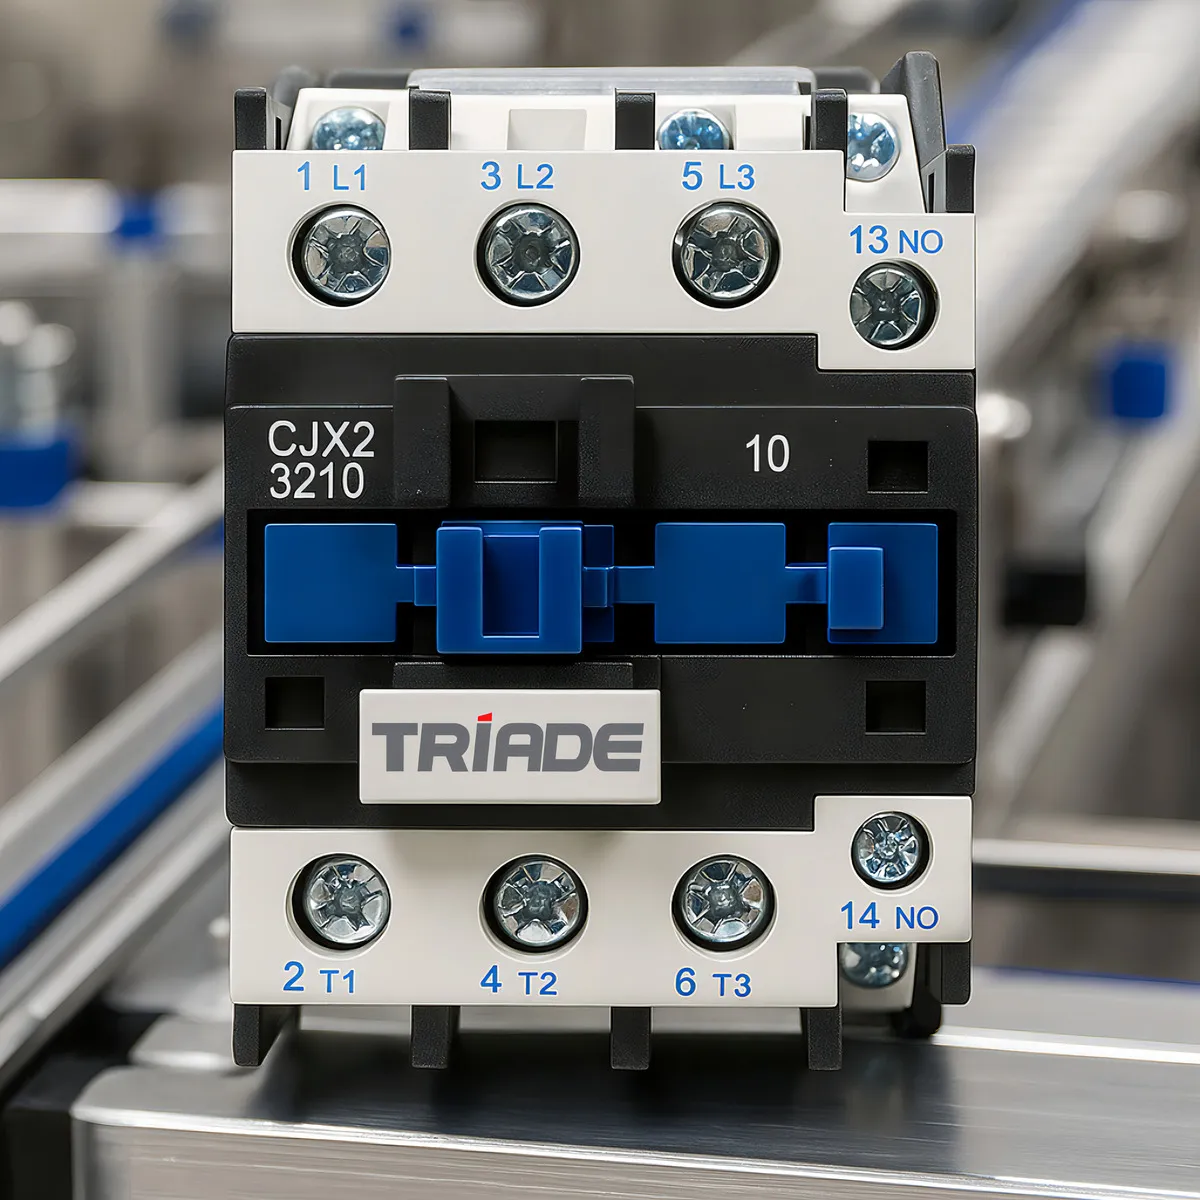
\includegraphics[width= 0.4\textwidth]{Figuras/contator.png} 
    \fonte{Figura extraída de \citeonline{ml_contator_cjx2}.} 
    \label{fig:Contactor} 
\end{figure}

Os contatores foram utilizados para o acionamento das cargas de maior potência, garantindo maior segurança elétrica e confiabilidade operacional. O controle desses dispositivos foi realizado indiretamente pelo microcontrolador por meio do módulo relé, que atua como interface de comando para a bobina do contator. Dessa forma, sinais de baixa potência provenientes do microcontrolador podem controlar cargas de maior potência de maneira segura, promovendo o isolamento entre o circuito de controle e o circuito de potência e reduzindo riscos associados à operação do sistema.

%------------------------------------------------------------------
\subsection{Integração e Ligações do Circuito}

A Figura \ref{fig:esquema_eletrico} apresenta o esquemático das conexões elétricas realizadas, detalhando a ligação entre o sensor PZEM-004T e o microcontrolador NodeMCU ESP8266, e do circuito de potência, incluindo relés, contatores e cargas. O módulo PZEM foi alimentado pelos pinos Vin e GND do NodeMCU. A comunicação entre os dispositivos ocorreu via interface serial UART, com conexão cruzada dos sinais: TX do PZEM ao RX do NodeMCU (GPIO 3) e RX do PZEM ao TX do NodeMCU (GPIO 1).

\begin{figure}[!htbp] 
    \centering
    \caption{Esquemático elétrico da aquisição de dados e controle de cargas.}
    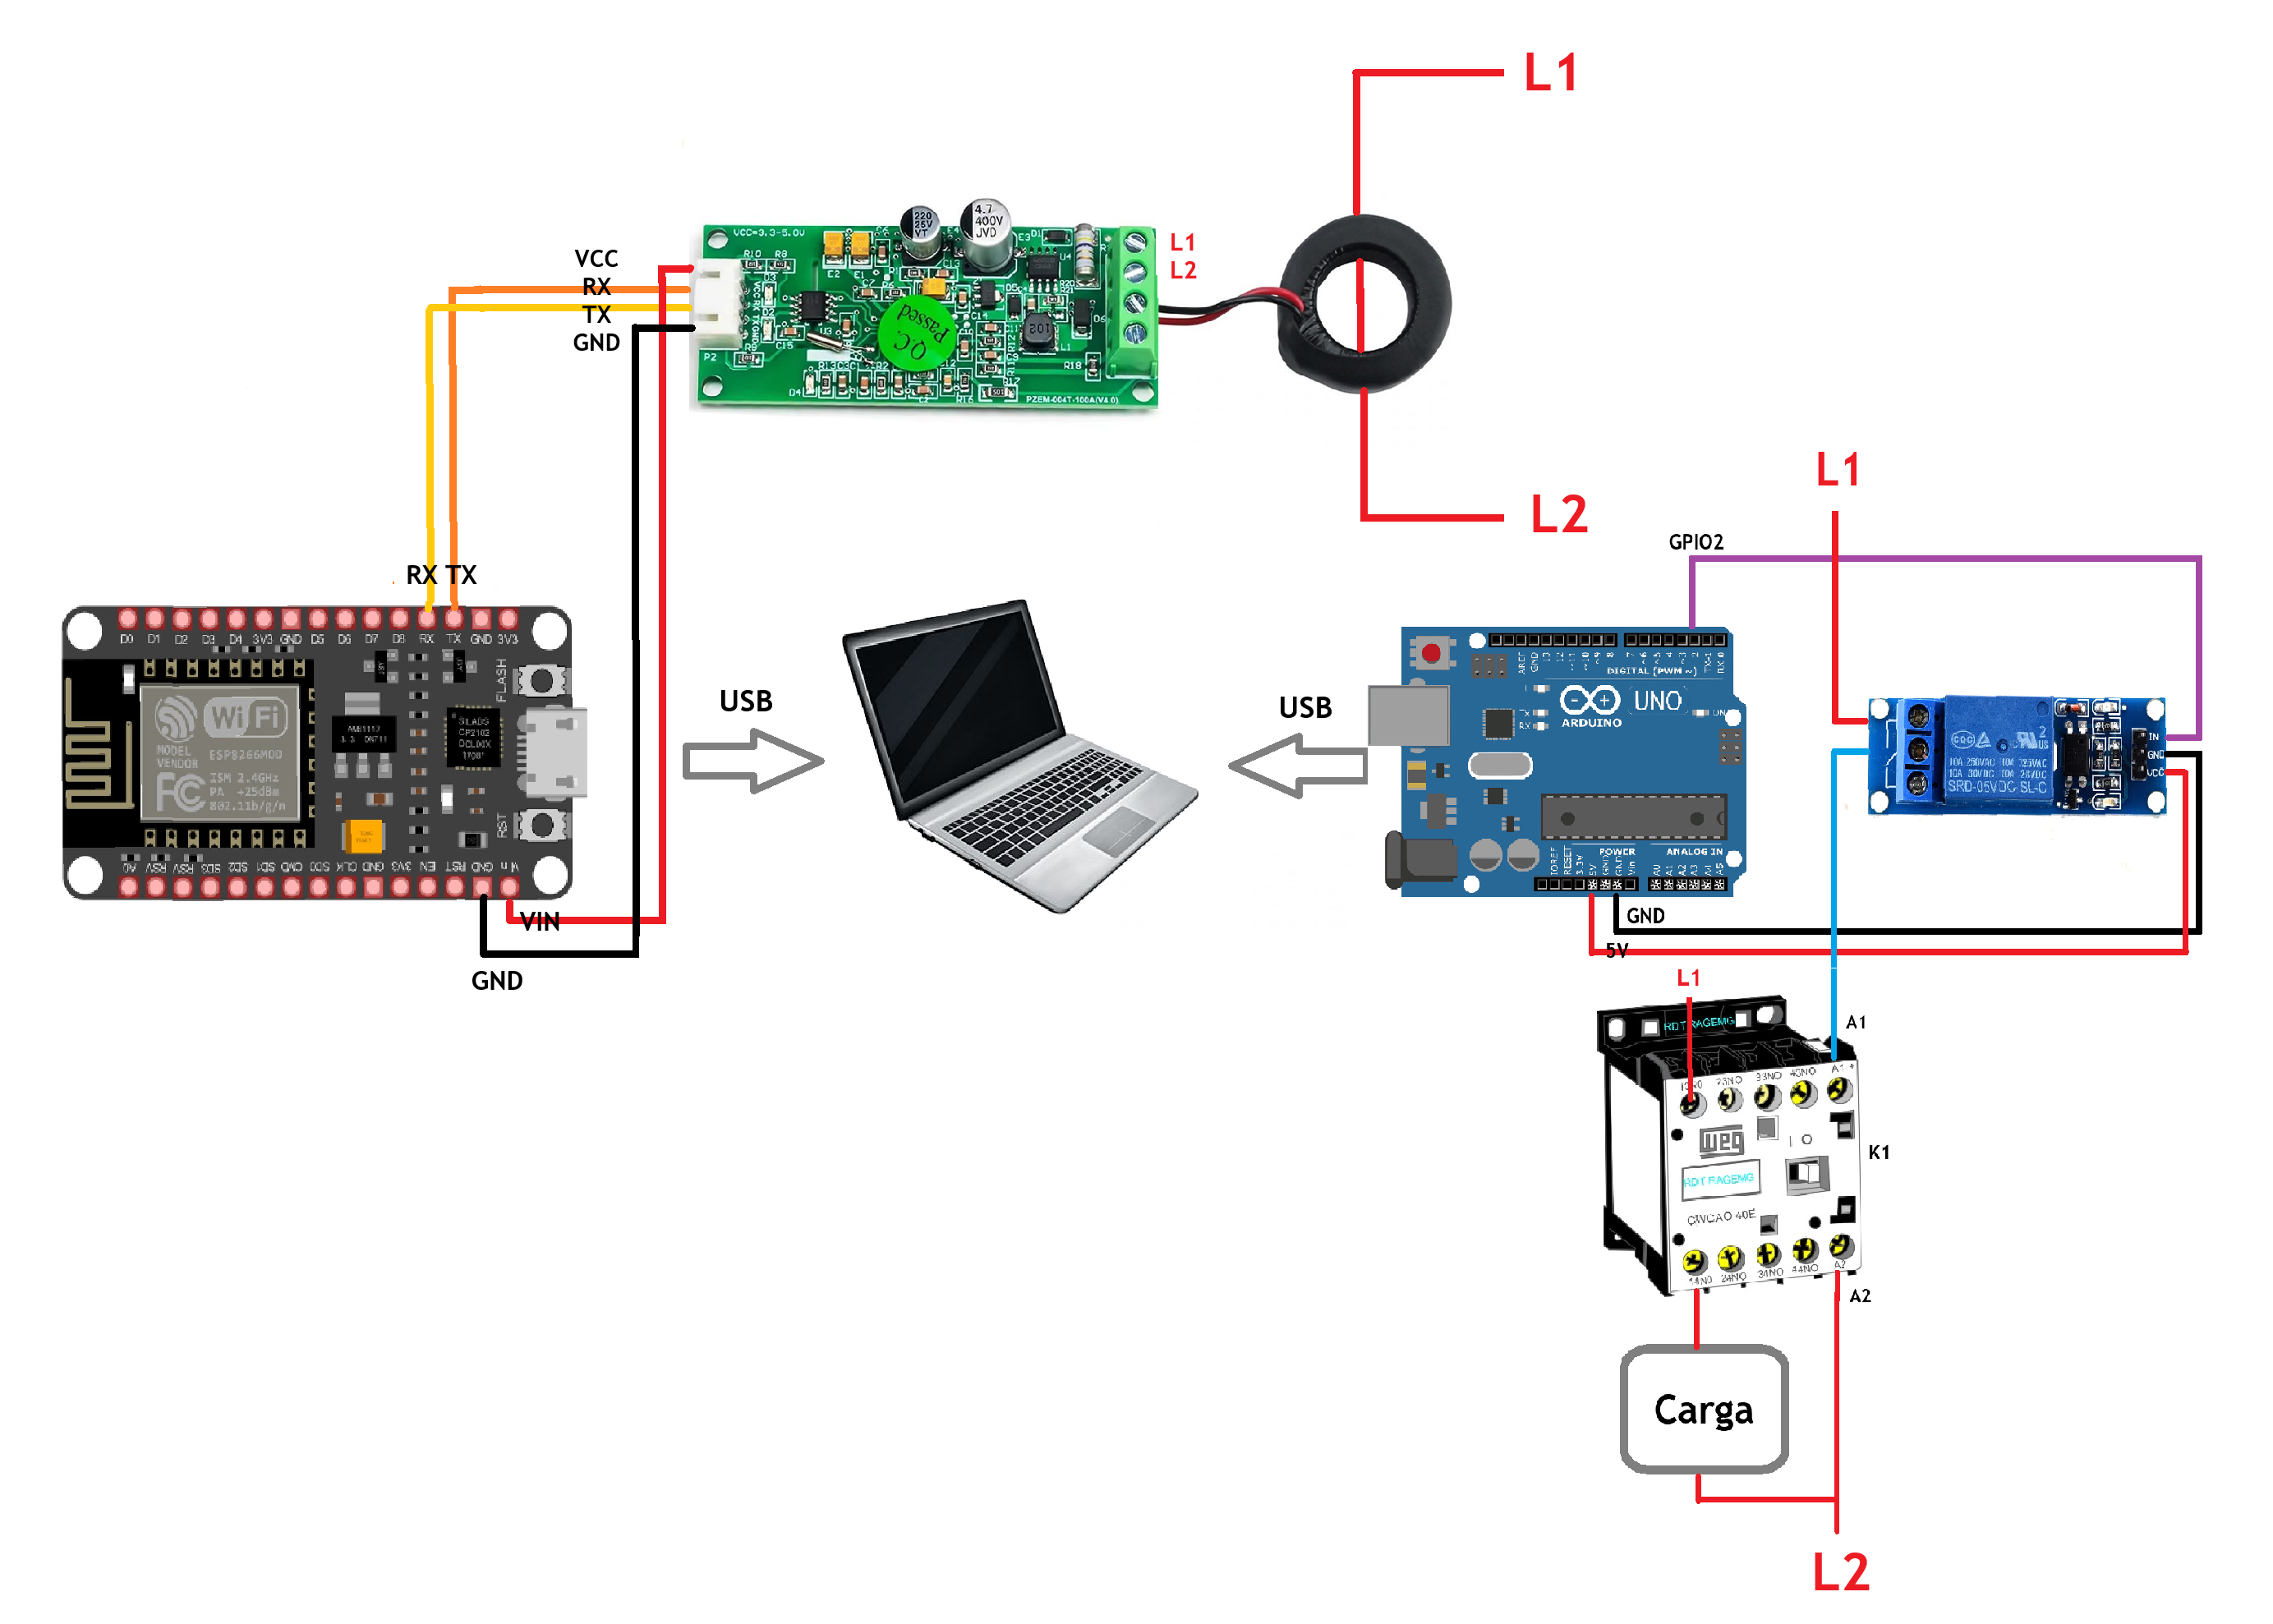
\includegraphics[width=1\textwidth]{Figuras/Esquematico_do_sistema (1).png} 
    \fonte{\me{2026}} 
    \label{fig:esquema_eletrico} 
\end{figure}

Essa arquitetura de conexão permitiu a leitura periódica das grandezas elétricas medidas pelo PZEM, possibilitando sua utilização tanto para armazenamento quanto para processamento pelos modelos implementados.

%------------------------------------------------------------------
%------------------------------------------------------------------
\section{Ambientes de Desenvolvimento e Implementação}

O Edge Impulse é uma plataforma de software especializada em soluções de Edge AI, voltada à simplificação do desenvolvimento e implantação de modelos de aprendizado de máquina, conforme ilustrado na Figura \ref{fig:edge_impulse}. A ferramenta oferece suporte completo ao ciclo de desenvolvimento de modelos de aprendizado de máquina, abrangendo etapas como aquisição de dados (com ou sem conectividade), pré-processamento, extração de características, treinamento, validação e exportação otimizada para execução em dispositivos ou ambientes de processamento \cite{STMicroelectronics}.

\begin{figure}[!htbp] 
    \centering
    \caption{Arquitetura da plataforma Edge Impulse.} 
    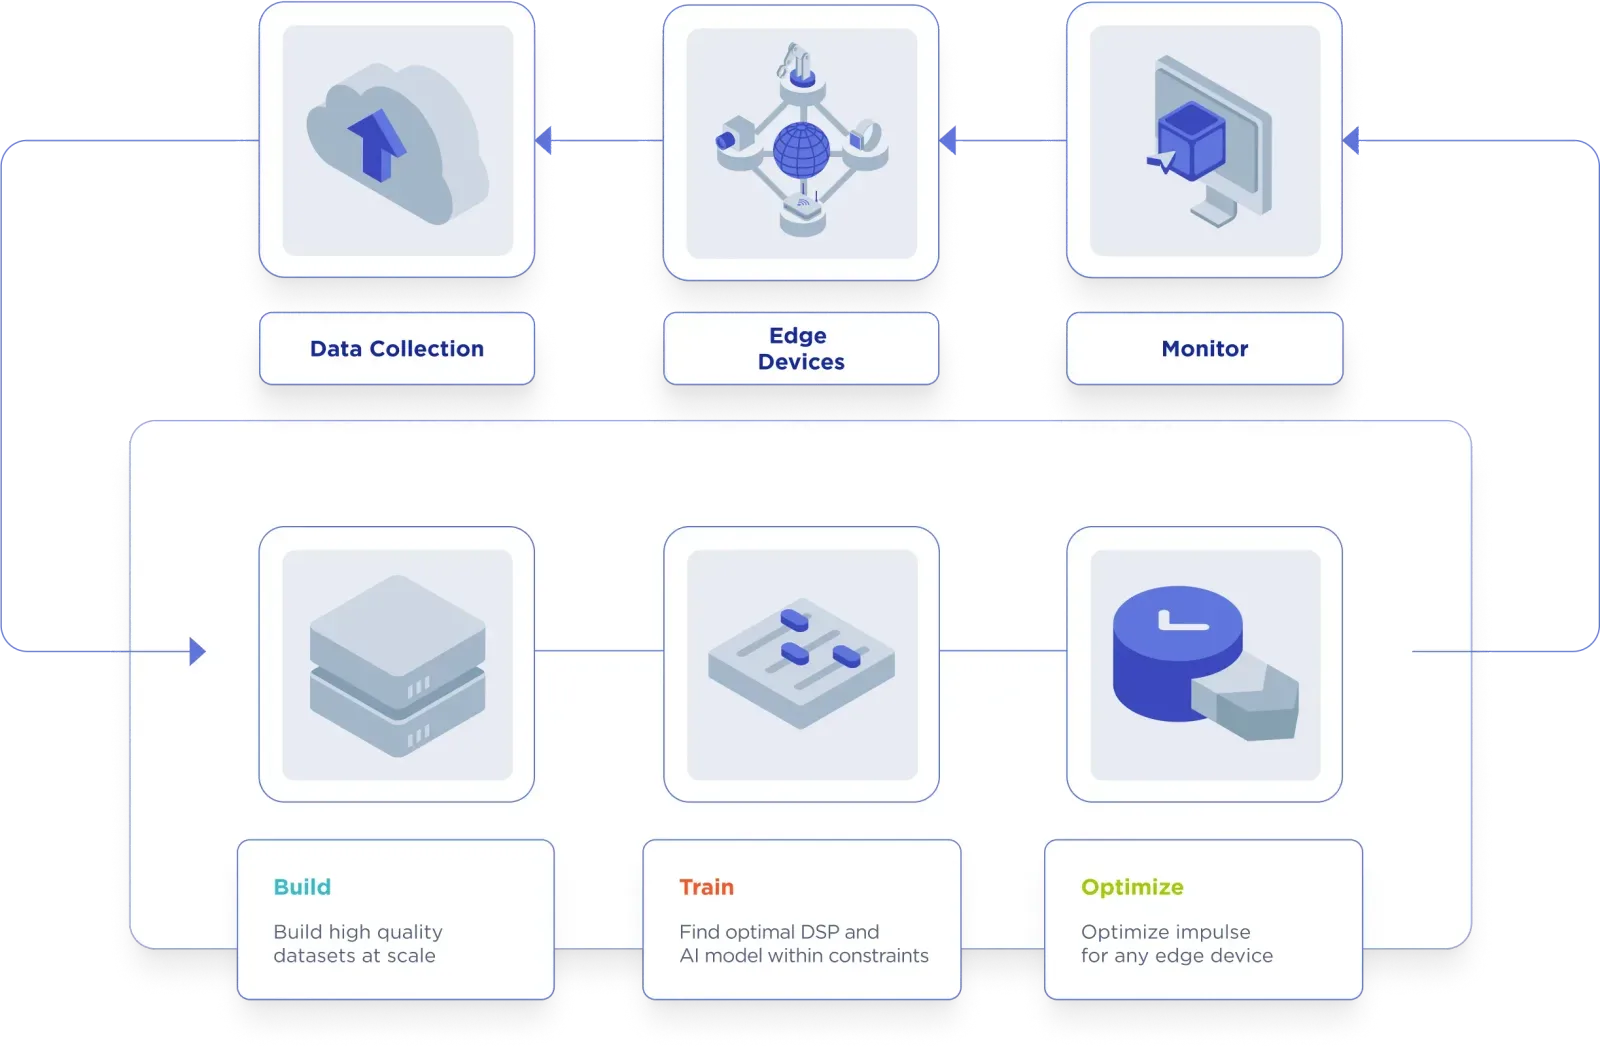
\includegraphics[width=1.0 \textwidth]{Figuras/Edge Impulse Diagrama.png} 
    \fonte{Figura extraída de \citeonline{STMicroelectronics}.} 
    \label{fig:edge_impulse} 
\end{figure}

Além da interface intuitiva e da facilidade de integração com diferentes plataformas de hardware e software, a ferramenta possibilita a realização de testes e otimizações utilizando dados reais, permitindo a identificação de inconsistências e ajustes no modelo antes de sua implantação final.

Neste trabalho, o Edge Impulse foi utilizado para a modelagem e treinamento de dois modelos baseados em redes neurais artificiais: um modelo de classificação, destinado à identificação do tipo de carga elétrica presente no sistema, e um modelo de regressão, utilizado para a estimativa do fator de potência (FP).

Os treinamentos dos modelos foram realizados em ambiente offline, utilizando dados históricos coletados durante os experimentos e previamente organizados em uma base de dados rotulada. A divisão do conjunto de dados em subconjuntos de treinamento e validação foi realizada dentro da própria plataforma Edge Impulse, permitindo a avaliação do desempenho dos modelos por meio de diferentes métricas. Após a etapa de treinamento e validação, os modelos foram exportados em formato compatível com execução em ambiente Node.js para integração no Node-RED.

O Node-RED foi utilizado para processamento e visualização dos dados em tempo real. No sistema proposto, a plataforma atua como cliente MQTT, conectando-se ao broker local para receber os dados medidos continuamente pelo sensor PZEM-004T e enviados pelo microcontrolador NodeMCU. Após o recebimento, os modelos exportados do Edge Impulse são executados no fluxo de processamento, realizando a inferência em tempo real e retornando os resultados, que são então exibidos em um dashboard web interativo desenvolvido para o acompanhamento das grandezas elétricas medidas e estimadas.

%------------------------------------------------------------------
\section{Modelagem e Treinamento dos Modelos}
\subsection{Geração da Base de Dados}
Para o treinamento dos modelos em ambiente Edge Impulse, foi necessário inicialmente construir uma base de dados rotulada representativa contendo as grandezas obtidas pelo sensor PZEM, bem como as grandezas derivadas calculadas a partir dessas medições, como potência aparente e potência reativa. Essas medições foram realizadas em bancada sob diferentes tipos de cargas em ambiente laboratorial controlado da Instituição.

Para essa etapa específica de aquisição de dados foi utilizado um microcontrolador Arduino Uno, empregado exclusivamente no controle das cargas, registro e armazenamento das medições em formato estruturado. Os códigos desenvolvidos para essa finalidade são apresentados nos Apêndices \ref{apendice_coleta_dados} e \ref{apendice_controle_cargas}.

Durante esse processo, os dados foram coletados em formato CSV, armazenados e organizados em uma planilha no \textit{Google Sheets}, apresentada no Apêndice \ref{apendice_google_sheets}, para posterior importação para o ambiente de treinamento dos modelos.

No total, foram coletadas 1000 amostras para cada tipo de carga, resultando em um conjunto de dados de 8000 amostras no total, para aplicação e avaliação dos modelos desenvolvidos. As classes de carga consideradas no processo de treinamento são apresentadas na Tabela \ref{tab_classes_carga}.

\begin{table}[!htbp]
    \centering
    \caption{Classes de carga utilizadas na base de dados}
    \label{tab_classes_carga}
    \begin{tabular}{|c|c|}
    \hline
    \textbf{Classe} & \textbf{Tipo de Carga} \\
    \hline
    0 & Sem carga \\
    \hline
    1 & Carga capacitiva \\
    \hline
    2 & Carga indutiva \\
    \hline
    3 & Carga resistiva \\
    \hline
    4 & Motor \\
    \hline
    5 & Cargas Resistiva + Capacitiva \\
    \hline
    6 & Cargas Resistiva + Indutiva \\
    \hline
    7 & Carga Capacitiva + Indutiva \\
    \hline
    \end{tabular}
    \fonte{\me{2026}}
\end{table}

\subsection{Pré-processamento dos Dados}

Antes do treinamento dos modelos, foi realizado o tratamento dos dados com o objetivo de melhorar a qualidade das informações fornecidas aos algoritmos de aprendizado de máquina.

Inicialmente, as variáveis de entrada foram submetidas a um processo de normalização utilizando o método \textit{StandardScaler}, que realiza a padronização com base na média e no desvio padrão da distribuição dos dados. Esse procedimento contribui para melhorar a convergência durante o treinamento das redes neurais. Posteriormente, o conjunto de dados foi dividido em dois subconjuntos: 80\% das amostras para treinamento e 20\% reservadas para teste e avaliação de desempenho.

\subsection{Configuração do Treinamento}
A Tabela \ref{tab_variaveis_modelo} apresenta as grandezas elétricas empregadas no treinamento dos modelos.

\begin{table}[!htbp]
    \centering
    \caption{Variáveis utilizadas no treinamento de cada modelo.}
    \label{tab_variaveis_modelo}
    \begin{tabular}{|c|c|c|}
    \hline
    \textbf{Modelo} & \textbf{Entradas}  & \textbf{Saídas} \\
    \hline
    Classificação & \makecell{Corrente, Potência Ativa, \\ Potência Aparente, Potência Reativa, \\ Fator de Potência} & Tipo de carga elétrica \\
    \hline
    Regressão & \makecell{Corrente, Potência Ativa, \\ Potência Aparente, Potência Reativa} & Fator de Potência \\
    \hline
    \end{tabular}
    \fonte{\me{2026}}
\end{table}


O treinamento foi realizado utilizando as ferramentas disponíveis na plataforma, com as seguintes configurações principais:
\begin{itemize}
    \item Número de épocas: 40
    \item Taxa de aprendizado (Learning rate): 0,0005
    \item Tamanho do conjunto de validação: 20\%
\end{itemize}

\subsection{Arquitetura da Rede Neural}

Os modelos de classificação e regressão foram implementados utilizando arquiteturas semelhantes de redes neurais do tipo MLP. Cada modelo é composto por uma camada de entrada correspondente às variáveis elétricas medidas, duas camadas intermediárias e uma camada de saída. A Tabela \ref{tab:arquitetura_modelos} apresenta a quantidade de neurônios utilizadas nas camadas de cada modelo.

\begin{table}[!htbp]
    \centering
    \caption{Arquitetura dos modelos de classificação e regressão.}
    \label{tab:arquitetura_modelos}
    \begin{tabular}{|c|c|c|}
    \hline
    \textbf{Camada} & \textbf{Classificação} & \textbf{Regressão} \\
    \hline
    Entrada & 5 & 4 \\
    \hline
    Oculta 1 & 20 & 20 \\
    \hline
    Oculta 2 & 30 & 30 \\
    \hline
    Saída & 8 & 1 \\
    \hline
    \end{tabular}
    \fonte{\me{2026}}
\end{table}

%------------------------------------------------------------------
%------------------------------------------------------------------
\section{Cenários de Aplicação e Validação dos Modelos}

As medições do sensor PZEM-004T foram lidas pelo microcontrolador NodeMCU ESP8266 e publicadas periodicamente no broker MQTT a cada 1 segundo em um tópico único denominado \textit{pzem/dados} no ambiente de processamento Node-RED. Para isso, foi necessário configurar as credenciais da rede Wi-Fi e do servidor MQTT utilizados para estabelecer a comunicação com o broker da aplicação. O código de integração entre o sensor PZEM-004T e o NodeMCU é apresentado no Apêndice \ref{cod_integracao_PZEM_MQTT}. 

Para a comunicação com o sensor foi utilizada a biblioteca \textit{PZEM004Tv30}, responsável por realizar a interface serial com o módulo de medição elétrica por meio da porta UART padrão do microcontrolador (GPIO1 e GPIO3). O programa também foi responsável por formatar os dados em um objeto no formato JSON para uso no Node-RED.

\subsection{Processamento no ambiente Node-RED}
Conforme apresentado na Figura \ref{fig:Nó edge-impulse-classify}, o ambiente Node-RED foi configurado como a camada responsável pelo processamento, integração e visualização do sistema, recebendo os dados enviados pelo microcontrolador via protocolo MQTT e executando os resultados dos modelos.

\begin{figure}[!htbp] 
    \centering
    \caption{Configuração do ambiente Node-RED.} 
    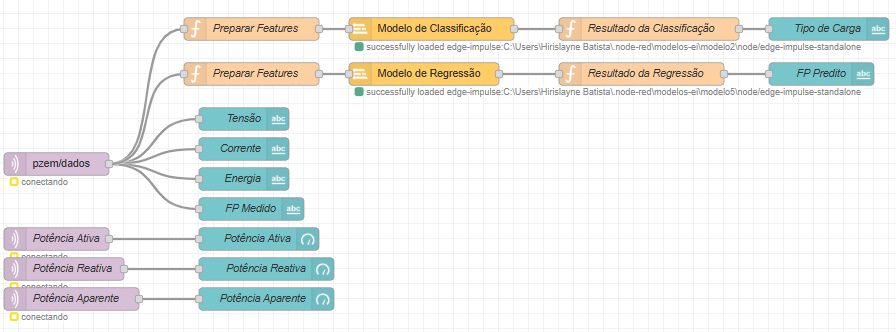
\includegraphics[width = 1\textwidth]{Figuras/Configuracao do Dashboard.png} 
    \fonte{\me{2026}} 
    \label{fig:Nó edge-impulse-classify} 
\end{figure}

As principais funcionalidades implementadas no fluxo de processamento são apresentadas na Tabela \ref{tab_fluxo_nodered}.

\begin{table}[!htbp]
    \centering
    \caption{Componentes do fluxo de processamento no Node-RED}
    \label{tab_fluxo_nodered}
    \begin{tabular}{|p{2.5cm}|p{5.5cm}|p{5.5cm}|}
    \hline
    \multicolumn{1}{|c|}{\textbf{Módulo}} & \multicolumn{1}{c|}{\textbf{Componente}} & \multicolumn{1}{c|}{\textbf{Função}} \\
    \hline
    Recepção & Nó MQTT IN (tópico \textit{pzem/dados}) & Recebe o JSON com todas as medições do sensor \\
    \hline
    Preparação & Nó Function \textit{Preparar Features} & Extrai e organiza as variáveis de entrada do modelo \\
    \hline
    Classificação e Estimativa & Nó \textit{edge-impulse-classify} & Executa o modelo \textit{WebAssembly} em tempo real \\
    \hline
    Processamento & Nós Functions \textit{Resultado da Classificação} e \textit{Resultado da Regressão} & Formatam os valores gerados pelos modelos para melhor visualização\\
    \hline
    Visualização & Nós \textit{text} e \textit{gauge} UI & Exibe medições, classificações e estimativas em tempo real \\
    \hline
    \end{tabular}
    \fonte{\me{2026}}
\end{table}

O nó \textit{Function} denominado \textit{Preparar Features} foi configurado para extrair do objeto JSON recebido via MQTT as variáveis necessárias para os modelos, organizando-as na mesma ordem utilizada durante o treinamento no Edge Impulse, conforme códigos apresentados em \ref{cod_preparacao_features_modelo_class} e \ref{cod_preparacao_features_modelo_regr}.

\begin{lstlisting}[language=JavaScript, caption={Preparação das variáveis de entrada para o modelo de classificação.}, label={cod_preparacao_features_modelo_class}]
    let dados = msg.payload;
    msg.payload = [
        Number(dados.corrente),
        Number(dados.potencia),
        Number(dados.aparente),
        Number(dados.reativa),
        Number(dados.fp)
    ];
    msg.dados = dados;
    return msg;
\end{lstlisting}

\begin{lstlisting}[language=JavaScript, caption={Preparação das variáveis de entrada para o modelo de regressão.}, label={cod_preparacao_features_modelo_regr}]
    let dados = msg.payload;
    msg.payload = [
        Number(dados.corrente),
        Number(dados.potencia),
        Number(dados.aparente),
        Number(dados.reativa)
    ];
    msg.dados = dados;
    return msg;
\end{lstlisting}

O nó \textit{edge-impulse-classify} foi configurado para executar cada um dos modelos. Para isso, basta copiar o caminho do diretório exportado do \textit{Edge Impulse} que contém os arquivos \textit{edge-impulse-standalone.js} e \textit{.wasm}, responsáveis pela execução do modelo de rede neural, e armazená-lo no diretório local do Node-RED, conforme a ilustrado na Figura \ref{fig:Nó edge-impulse-classify}.

\begin{figure}[!htbp] 
    \centering
    \caption{Configuração do nó \textit{edge-impulse-classify}.} 
    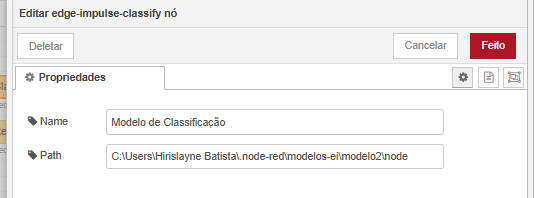
\includegraphics[width = 1\textwidth]{Figuras/Nó edge-impulse-classify.png} 
    \fonte{\me{2026}} 
    \label{fig:Nó edge-impulse-classify} 
\end{figure}

A cada novo conjunto de dados recebido, os nós executam o processo de inferência e retornam as probabilidades associadas a cada uma das oito classes de carga e o valor do FP estimado, respectivamente, enviando esses valores para os nós de função seguintes, denominados \textit{Resultado da Classificação} e \textit{Resultado da Regressão}.  Esses resultados são então enviados para os nós de função seguintes, denominados \textit{Resultado da Classificação} e \textit{Resultado da Regressão}, que interpretam e formatam as saídas para o dashboard. Os códigos referentes a essas funções são apresentados em \ref{cod_resultado_classificacao} e \ref{cod_resultado_regressao}.

\begin{lstlisting}[language=JavaScript, caption={Processamento da saída do modelo de classificação}, label={cod_resultado_classificacao}]
    // recebe a saida do Edge Impulse
    let resultados = msg.payload.results;
    
    // cria um texto formatado para o dashboard
    let classe = "";
    let maior = 0;
    
    // percorre todas as classes
    for (let i = 0; i < resultados.length; i++) {
        if (resultados[i].value > maior) {
            maior = resultados[i].value;
            classe = resultados[i].label;
        }
    }
    
    let nomes = {
        "0": "Sem carga",
        "1": "Capacitiva",
        "2": "Indutiva",
        "3": "Resistiva",
        "4": "Motor",
        "5": "Resistiva + Capacitiva",
        "6": "Resisitiva + Indutiva",
        "7": "Capacitiva + Indutiva"
    };
    
    msg.payload = nomes[classe];
    return msg;
\end{lstlisting}

\begin{lstlisting}[language=JavaScript, caption={Processamento da saída do modelo de regressão.}, label={cod_resultado_regressao}]
    let resultados = msg.payload.results;
    let valor = 0;
    valor = resultados[0].value;
    
    msg.payload = valor;
    return msg;
\end{lstlisting}

Por fim, as medições e os resultados dos modelos foram disponibilizados em um painel de monitoramento desenvolvido na plataforma Node-RED, conforme exemplo ilustrado na Figura \ref{fig:painel-monitoramento}. Esse painel permite a visualização em tempo real das grandezas medidas pelo sensor, da classe de carga identificada e do fator de potência estimado, por meio de elementos visuais como gráficos e indicadores textuais.

\begin{figure}[!htbp] 
    \centering
    \caption{ Painel de monitoramento Node-RED.} 
    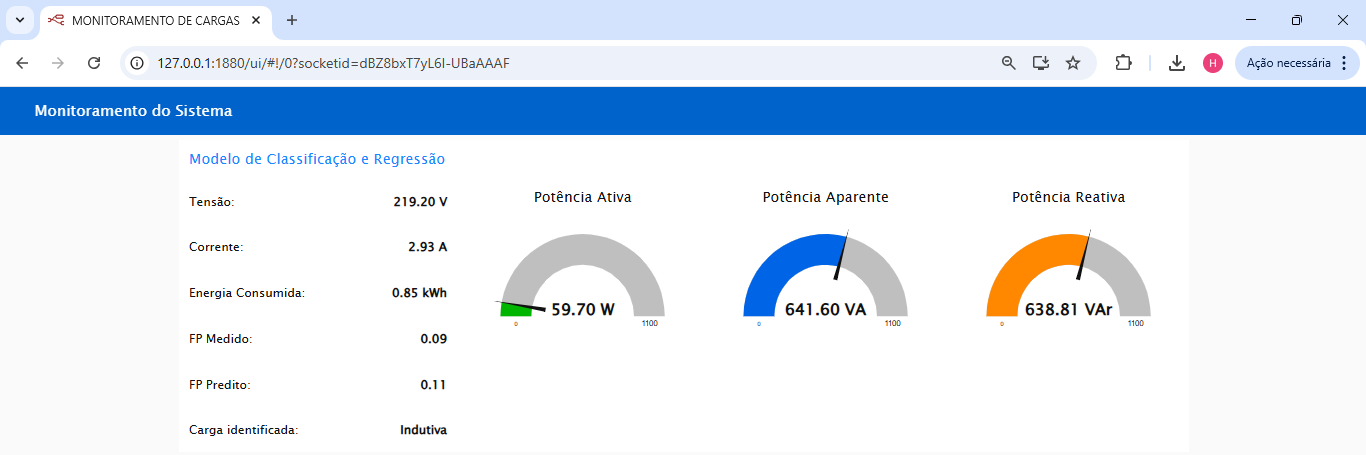
\includegraphics[width = 1\textwidth]{Figuras/tela_carga_indutiva.png} 
    \fonte{\me{2026}} 
    \label{fig:painel-monitoramento} 
\end{figure}